\documentclass[aspectratio=169,notes]{beamer}
\usepackage{lmodern}
\usepackage{adjustbox}
\usepackage[T1]{fontenc}
\usepackage{textcomp}
\usepackage{animate}
\usepackage{underscore}
\usepackage{pdfpc-commands}
\usepackage{xmpmulti}
\usepackage{multimedia}
\usepackage{epstopdf}
\usepackage{bbding}
\usepackage{standalone}

\definecolor{Title}{rgb}{0.94,0.52,0.08}
\setbeamercolor{frametitle}{bg=Title,fg=black}

% footnote without number
\makeatletter
\def\blfootnote{\xdef\@thefnmark{}\@footnotetext}
\makeatother

\usepackage{hyperref}
\usepackage{scalerel}
\def\thumbup{\scalerel*{\includegraphics{thumbup.png}}{O}}
\usepackage{listings}
\lstdefinelanguage{D}
{
  % list of keywords
  morekeywords={ abstract, alias, align, asm, assert, auto, body, bool, break,
	byte, case, cast, catch, cdouble, cent, cfloat, char, class, const,
	continue, default, double, else, enum, export, extern, false, final, finally,
	float, for, foreach, foreach_reverse, function, goto, idouble, if, ifloat,
	immutable, import, in, inout, int, interface, invariant, ireal, is, lazy,
	long, mixin, module, new, nothrow, null, out, override, package, pragma,
	private, protected, public, pure, real, ref, return, scope, shared, short,
	static, string, struct, super, switch, synchronized, template, this, throw,
	true, try, typeid, typeof, ubyte, ucent, uint, ulong, union,
	unittest, delegate, @safe, @property
	ushort, version, void, wchar, while, with, __FILE__, __FILE_FULL_PATH__,
	__MODULE__, __LINE__, __FUNCTION__, __PRETTY_FUNCTION__, __gshared,
	__traits, __vector, __parameters
  },
  otherkeywords= { @property, @safe },
  sensitive=false, % keywords are not case-sensitive
  morecomment=[l]{//}, % l is for line comment
  morecomment=[s]{/*}{*/}, % s is for start and end delimiter
  morecomment=[s]{/+}{+/}, % s is for start and end delimiter
  morestring=[b]" % defines that strings are enclosed in double quotes
}
\usepackage{color}
\definecolor{eclipseBlue}{RGB}{42,0.0,255}
\definecolor{eclipseGreen}{RGB}{63,127,95}
\definecolor{eclipsePurple}{RGB}{127,0,85}

% Set Language
\lstset{
  language={D},
  basicstyle=\small\ttfamily, % Global Code Style
  captionpos=b, % Position of the Caption (t for top, b for bottom)
  extendedchars=true, % Allows 256 instead of 128 ASCII characters
  tabsize=2, % number of spaces indented when discovering a tab 
  columns=fixed, % make all characters equal width
  keepspaces=true, % does not ignore spaces to fit width, convert tabs to spaces
  showstringspaces=false, % lets spaces in strings appear as real spaces
  breaklines=true, % wrap lines if they don't fit
  numbers=left, % show line numbers at the left
  numberstyle=\tiny\ttfamily, % style of the line numbers
  commentstyle=\color{eclipseGreen}, % style of comments
  keywordstyle=\color{eclipsePurple}, % style of keywords
  stringstyle=\color{eclipseBlue}, % style of strings
}
\definecolor{lightgray}{rgb}{.9,.9,.9}
\definecolor{darkgray}{rgb}{.4,.4,.4}
\definecolor{purple}{rgb}{0.65, 0.12, 0.82}
\lstdefinelanguage{TypeScript}{
	keywords={break, case, catch, continue, debugger, default, delete, do, else,
		false, from, finally, for, function, if, in, instanceof, new, null, return, switch,
		this, throw, true, try, typeof, var, void, while, with, interface,
		class, export, boolean, throw, implements, import, this, const, let,
		of, =>},
	morecomment=[l]{//},
	morecomment=[s]{/*}{*/},
	morestring=[b]',
	morestring=[b]",
	ndkeywords={},
	keywordstyle=\color{blue}\bfseries,
	ndkeywordstyle=\color{darkgray}\bfseries,
	identifierstyle=\color{black},
	commentstyle=\color{purple}\ttfamily,
	stringstyle=\color{red}\ttfamily,
	sensitive=true
}

\colorlet{punct}{red!60!black}
\definecolor{background}{HTML}{EEEEEE}
\definecolor{delim}{RGB}{20,105,176}
\colorlet{numb}{magenta!60!black}

\lstdefinelanguage{GraphQL}{
    basicstyle=\normalfont\ttfamily,
    numbers=left,
    stepnumber=1,
    showstringspaces=false,
    breaklines=true,
	keywords={type, schema, mutation, subscription, __type, __schema, kind,
		on, fragment, query},
    literate=
     *{0}{{{\color{numb}0}}}{1}
      {1}{{{\color{numb}1}}}{1}
      {2}{{{\color{numb}2}}}{1}
      {3}{{{\color{numb}3}}}{1}
      {4}{{{\color{numb}4}}}{1}
      {5}{{{\color{numb}5}}}{1}
      {6}{{{\color{numb}6}}}{1}
      {7}{{{\color{numb}7}}}{1}
      {8}{{{\color{numb}8}}}{1}
      {9}{{{\color{numb}9}}}{1}
      {:}{{{\color{punct}{:}}}}{1}
      {,}{{{\color{punct}{,}}}}{1}
      {\{}{{{\color{delim}{\{}}}}{1}
      {\}}{{{\color{delim}{\}}}}}{1}
      {[}{{{\color{delim}{[}}}}{1}
      {]}{{{\color{delim}{]}}}}{1},
}

\lstdefinelanguage{json}{
    basicstyle=\normalfont\ttfamily,
    numbers=left,
    stepnumber=1,
    showstringspaces=false,
    breaklines=true,
    literate=
     *{0}{{{\color{numb}0}}}{1}
      {1}{{{\color{numb}1}}}{1}
      {2}{{{\color{numb}2}}}{1}
      {3}{{{\color{numb}3}}}{1}
      {4}{{{\color{numb}4}}}{1}
      {5}{{{\color{numb}5}}}{1}
      {6}{{{\color{numb}6}}}{1}
      {7}{{{\color{numb}7}}}{1}
      {8}{{{\color{numb}8}}}{1}
      {9}{{{\color{numb}9}}}{1}
      {:}{{{\color{punct}{:}}}}{1}
      {,}{{{\color{punct}{,}}}}{1}
      {\{}{{{\color{delim}{\{}}}}{1}
      {\}}{{{\color{delim}{\}}}}}{1}
      {[}{{{\color{delim}{[}}}}{1}
      {]}{{{\color{delim}{]}}}}{1},
}
\usepackage{tikz}
\usetikzlibrary{shadows,calc}
\usepackage{xkeyval}
\usepackage{todonotes}
\presetkeys{todonotes}{inline}{}
\defbeamertemplate{description item}{align left}{\insertdescriptionitem\hfill}
\usetheme{metropolis}					 % Use metropolis theme
\usepackage[
    backend=biber,
	sorting=none,
    url=true 
]{biblatex}
\addbibresource{biblio.bib}
\setbeamertemplate{bibliography item}{\insertbiblabel}

\title{D The functional programming language\\nobody is talking about}
\date{\today}
\author{Robert Schadek}
\begin{document}
	\maketitle

	\begin{frame}[fragile]{D is a functional programming language}
		\begin{center}
			{\large What makes D a functional programming language}
		\end{center}
	\end{frame}

	\begin{frame}{C the functional programming language}
		\begin{itemize}
			\item D is a $\approx$ superset of C
			\item C is a functional programming language
		\end{itemize}
	\end{frame}

	\section{Proof by example}
	\begin{frame}[fragile]{High order functions}
		\lstinputlisting[language=C,basicstyle=\normalsize\ttfamily]{chof.c}
	\end{frame}

	\begin{frame}[fragile]{High order functions}
		\lstinputlisting[language=C,basicstyle=\normalsize\ttfamily]{chof2.c}
	\end{frame}

	\begin{frame}[fragile]{High order functions}
		\lstinputlisting[language=D,basicstyle=\normalsize\ttfamily]{dhof.d}
	\end{frame}

	\begin{frame}[fragile]{High order functions}
		\lstinputlisting[language=D,basicstyle=\normalsize\ttfamily]{dhof2.d}
	\end{frame}

	\section{Why should you care}
	\begin{frame}[fragile]{Why should you care about D}
\begin{center}
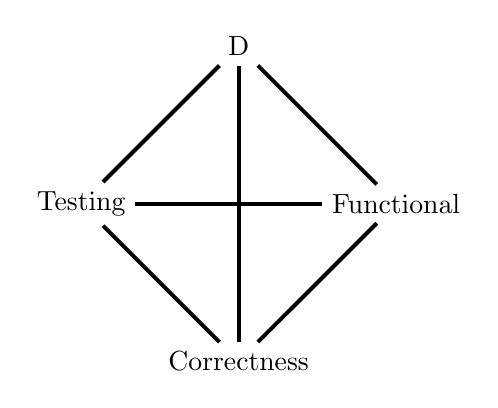
\begin{tikzpicture}[
	level 1/.style={sibling distance=3cm},
	level 2/.style={sibling distance=1cm},
	level 3/.style={sibling distance=0.5cm},
	%every node/.style = {shape=circle,
    %draw, align=center,minimum width=0.75cm,
    %top color=white, bottom color=blue!20}
]
]
	\node[] at (0.0,2.0) (0) {D};
	\node[] at (2.0,0.0) (1) {Functional};
	\node[] at (-2.0,0.0) (2) {Testing};
	\node[] at (0.0,-2.0) (3) {Correctness};

	\draw[-,line width=0.5mm,black] (0) -- (1);
	\draw[-,line width=0.5mm,black] (1) -- (2);
	\draw[-,line width=0.5mm,black] (0) -- (2);
	\draw[-,line width=0.5mm,black] (0) -- (3);
	\draw[-,line width=0.5mm,black] (2) -- (3);
	\draw[-,line width=0.5mm,black] (1) -- (3);
		\end{tikzpicture}
\end{center}
	\end{frame}

	\begin{frame}[fragile]{Why should you care}
		\lstinputlisting[firstline=6,lastline=18,language=D,basicstyle=\small\ttfamily]{rng2.d}
	\end{frame}

	\section{Ranges Ranges Ranges}
	\begin{frame}[fragile]{Ranges Ranges Ranges}
		\begin{center}
			A thing \lstinline@foreach@ can iterate
		\end{center}
	\end{frame}

	\begin{frame}[fragile]{Ranges}
		\lstinputlisting[firstline=3,lastline=18,language=D,basicstyle=\small\ttfamily]{rng1.d}
	\end{frame}

	\begin{frame}[fragile]{Ranges}
		\lstinputlisting[firstline=20,lastline=24,language=D,basicstyle=\small\ttfamily]{rng1.d}
		\pause
		\lstinputlisting[firstline=26,lastline=32,language=D,basicstyle=\small\ttfamily]{rng1.d}
	\end{frame}

	\begin{frame}[fragile]{Range types}
		\begin{itemize}
			\item Input Range
				\pause
			\item Forwared Range
			\begin{itemize}
				\item \lstinline@save()@
			\end{itemize}
			\item Bidirectional Range
			\begin{itemize}
				\item \lstinline@back@
				\item \lstinline@popBack@
			\end{itemize}
			\item Random Access Range
			\begin{itemize}
				\item \lstinline@[]@
			\end{itemize}
			\item Infinite Range
			\begin{itemize}
				\item \lstinline@enum empty = false;@
			\end{itemize}
		\end{itemize}\mbox{}\\[1cm]
	\end{frame}
	\begin{frame}[fragile]{Ranges types, practically}
		\lstinputlisting[firstline=35,lastline=37,language=D,basicstyle=\small\ttfamily]{rng1.d}
	\end{frame}

	\begin{frame}[fragile]{Ranges}
		\lstinputlisting[firstline=40,lastline=54,language=D,basicstyle=\small\ttfamily]{rng1.d}
	\end{frame}

	\begin{frame}[fragile]{Ranges}
		\lstinputlisting[firstline=56,lastline=63,language=D,basicstyle=\small\ttfamily]{rng1.d}
	\end{frame}

	\begin{frame}[fragile]{Ranges}
		\lstinputlisting[firstline=65,lastline=79,language=D,basicstyle=\small\ttfamily]{rng1.d}
	\end{frame}

	\begin{frame}[fragile]{Ranges}
		\lstinputlisting[firstline=81,lastline=90,language=D,basicstyle=\small\ttfamily]{rng1.d}
	\end{frame}

	\begin{frame}[fragile]{Uniform functional call syntax (UFCS)}
		\lstinputlisting[firstline=1,lastline=12,language=D,basicstyle=\small\ttfamily]{ufcs.d}
	\end{frame}

	\begin{frame}[fragile]{Ranges}
		\lstinputlisting[firstline=6,lastline=18,language=D,basicstyle=\small\ttfamily]{rng2.d}
	\end{frame}

	\section{Testing}
	\begin{frame}[fragile]{Testing}
		\begin{center}
		\Large Not tests $=$ wrong
		\end{center}
	\end{frame}

	\begin{frame}[fragile]{Testing in D}
		\begin{itemize}
			\item D has in-build unittesting
			\item \lstinline@unittest { }@
			\item D has in-build test coverage analysis
			\item 100\% is a terrible metric, but still the best we have
		\end{itemize}
	\end{frame}

	\begin{frame}[fragile]{Coverage analysis}
		\lstinputlisting[firstline=1,lastline=8,language=D,basicstyle=\small\ttfamily]{cov.d}
		dmd -main -cov -unittest -run cov.d
	\end{frame}

	\begin{frame}[fragile]{Coverage analysis}
		\lstinputlisting[firstline=1,lastline=8,language=D,basicstyle=\small\ttfamily]{cov.lst}
	\end{frame}

	\begin{frame}[fragile]{Coverage analysis}
		\lstinputlisting[firstline=10,lastline=19,language=D,basicstyle=\small\ttfamily]{cov.d}
	\end{frame}

	\begin{frame}[fragile]{Coverage analysis}
		\lstinputlisting[firstline=10,lastline=19,language=D,basicstyle=\small\ttfamily]{cov.lst}
	\end{frame}

	\begin{frame}[fragile]{Coverage analysis}
		\lstinputlisting[firstline=21,lastline=27,language=D,basicstyle=\small\ttfamily]{cov.d}
	\end{frame}

	\begin{frame}[fragile]{Coverage analysis}
		\mbox{}\\[2cm]
		\lstinputlisting[firstline=21,lastline=27,language=D,basicstyle=\small\ttfamily]{cov.lst}
	\end{frame}

	\begin{frame}[fragile]{Coverage analysis}
		\lstinputlisting[firstline=29,lastline=42,language=D,basicstyle=\small\ttfamily]{cov.lst}
	\end{frame}

	\section{Exceptions}
	{
	\usebackgroundtemplate{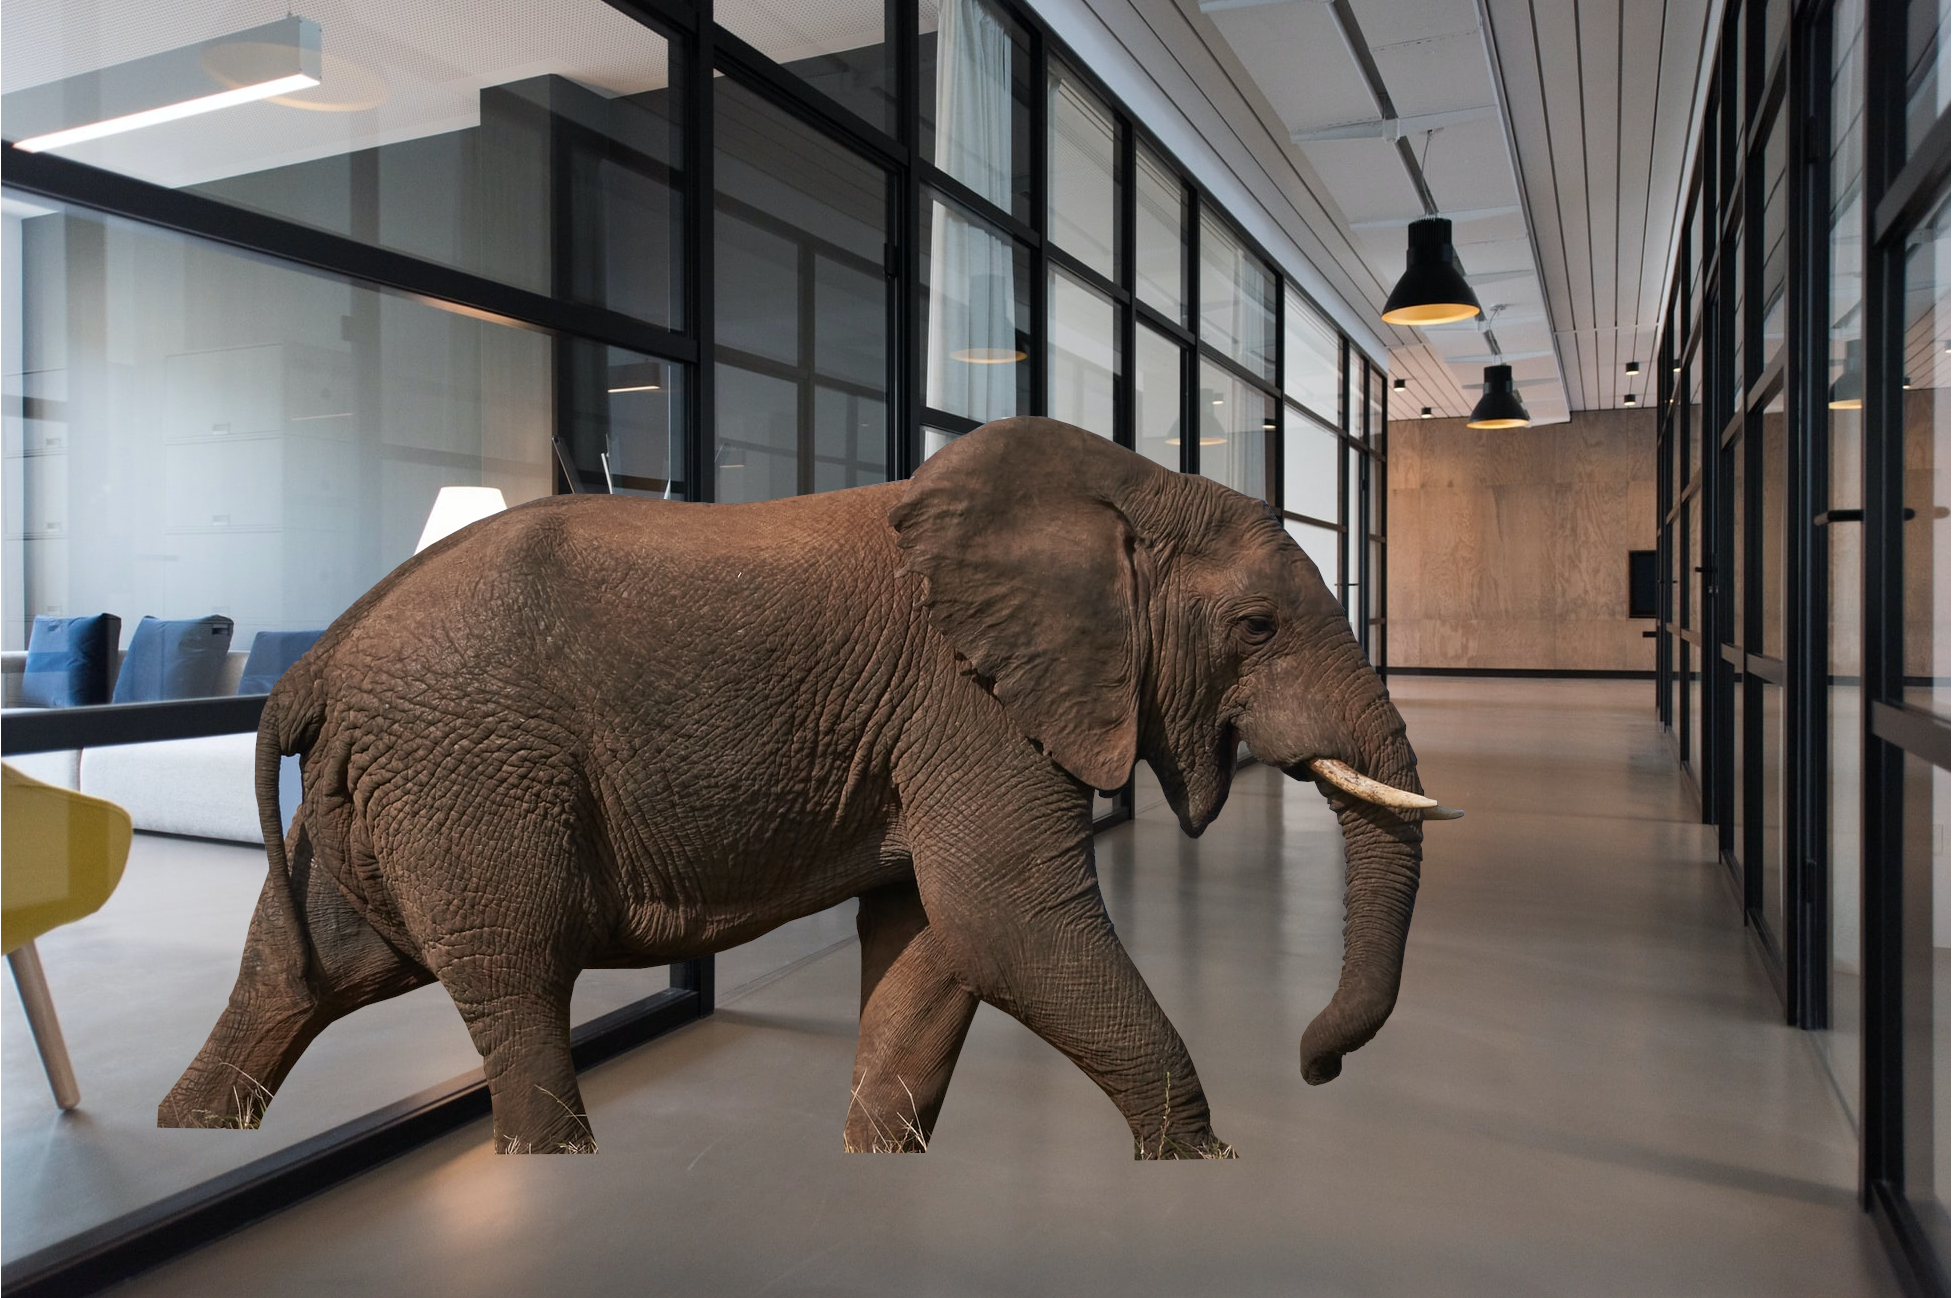
\includegraphics[width=\paperwidth]{elephant.png}}
	\begin{frame}[fragile]{Elephant in the Room}
	\end{frame}
	}

	\begin{frame}[fragile]{Elephant in the Room}
		\lstinputlisting[firstline=4,lastline=19,language=D,basicstyle=\small\ttfamily]{exp.d}
	\end{frame}

	\begin{frame}[fragile]{handle Exceptions}
		\lstinputlisting[firstline=22,lastline=27,language=D,basicstyle=\small\ttfamily]{exp.d}
	\end{frame}

	\begin{frame}[fragile]{try catch}
		\lstinputlisting[firstline=33,lastline=45,language=D,basicstyle=\small\ttfamily]{exp.d}
	\end{frame}

	\begin{frame}[fragile]{try catch nullable}
		\lstinputlisting[firstline=52,lastline=66,language=D,basicstyle=\small\ttfamily]{exp.d}
	\end{frame}

	\section{State}

	\begin{frame}[fragile]{State}
		\begin{itemize}
			\item Most programs are not just input, map, output
			\item Most programs have some sort of state
		\end{itemize}
	\end{frame}

	\begin{frame}[fragile]{State: The model}
		\lstinputlisting[firstline=3,lastline=11,language=D,basicstyle=\small\ttfamily]{state.d}
	\end{frame}

	\begin{frame}[fragile]{State: \lstinline{createGroup}}
		\lstinputlisting[firstline=13,lastline=27,language=D,basicstyle=\small\ttfamily]{state.d}
	\end{frame}

	\begin{frame}[fragile]{State: \lstinline{findGroup}}
		\lstinputlisting[firstline=29,lastline=39,language=D,basicstyle=\small\ttfamily]{state.d}
	\end{frame}

	\begin{frame}[fragile]{State: \lstinline{addMember}}
		\lstinputlisting[firstline=41,lastline=53,language=D,basicstyle=\small\ttfamily]{state.d}
	\end{frame}

	\begin{frame}[fragile]{State: Usage}
		\lstinputlisting[firstline=55,lastline=63,language=D,basicstyle=\small\ttfamily]{state.d}
	\end{frame}

	\begin{frame}[fragile]{State Two: \lstinline{createGroup}}
		\lstinputlisting[firstline=36,lastline=52,language=D,basicstyle=\small\ttfamily]{state2.d}
	\end{frame}

	\begin{frame}[fragile]{State Two: \lstinline{addMember}}
		\lstinputlisting[firstline=66,lastline=78,language=D,basicstyle=\small\ttfamily]{state2.d}
	\end{frame}

	\begin{frame}[fragile]{State Two: \lstinline{deepCopy} 1/2}
		\lstinputlisting[firstline=3,lastline=13,language=D,basicstyle=\small\ttfamily]{state2.d}
	\end{frame}

	\begin{frame}[fragile]{State Two: \lstinline{deepCopy} 2/2}
		\lstinputlisting[firstline=14,lastline=24,language=D,basicstyle=\small\ttfamily]{state2.d}
	\end{frame}

	\begin{frame}[fragile]{Commercial break}
		\begin{center}
			{\Large Symmetry Investments}
		\end{center}
	\end{frame}

	\section{Conclusion}
	\begin{frame}[fragile]{Takeaways}
		\begin{itemize}
			\item \lstinline{if} statements considered harmful
			\item learn phobos/std by heart
			\item when you think exception \lstinline{goto} Nullable
			\item no tests $=$ bugs
		\end{itemize}
	\end{frame}

	\section{The End}

	\section{Encore}

	\begin{frame}[fragile]{Dead lock free multi Mutex Systems}
		Deadlock Recipe:\\
		\begin{itemize}
			\item Mutual exclusion
			\item Hold and wait
			\item No preemption
			\item Circular wait
		\end{itemize}
	\end{frame}

	\begin{frame}[fragile]{Anti Dead lock: Un-sorted}
		\includestandalone[width=0.4\textwidth]{dl}
	\end{frame}

	\begin{frame}[fragile]{Anti Dead lock: Sorted}
		\includestandalone[width=0.4\textwidth]{dl2}
	\end{frame}

	\begin{frame}[fragile]{Anti Dead lock}
		\lstinputlisting[firstline=1,lastline=7,language=D,basicstyle=\small\ttfamily]{deadlock.d}
		\pause
		\lstinputlisting[firstnumber=8,firstline=8,lastline=15,language=D,basicstyle=\small\ttfamily]{deadlock.d}
	\end{frame}

	\section{Out of Slides}
\end{document}
